%!TEX root = ./qualification.tex

\newpage
\section{Capítulo 2 - Algorítmos Genéticos}
A programação genética baseia-se no princípio de reprodução e sobrevivência dos mais aptos de Charles Darwin, simulando o processo biológico de evolução. Existem diversas características que são comuns tanto ao processo evolutivo biológico quanto a problemas computacionais. A evolução pode ser entendida como um método de busca em uma vasta quantidade de indivíduos de diversas espécies diferentes, de modo adaptativo -  sofrendo alterações conforme o ambiente, população, características pessoais, etc. Esse tipo de busca é comumente encontrado em vários problemas computacionais onde precisamos examinar uma enorme massa de dados afim de encontrar boas respostas para determinado problema, respondendo satisfatoriamente a mudanças de ambiente.

Existem diversas áreas de aplicação, podendo-se destacar: otimização (propósito deste trabalho), programação automática, aprendizado de máquina, modelos econômicos, sociais e ecológicos, interações entre evolução e aprendizado, etc.

A abstração da evolução biológica feita por John Holland na década de 1960 tem como objetivo encontrar a melhor solução para determinado problema  deslocando-se por diversas gerações de uma população a outra de cromossomos utilizando a seleção juntamente com mecanismos de reprodução e mutação.

Algorítmos Genéticos funcionam descobrindo, destacando e recombinando bons blocos de soluções de forma altamente paralela. \cite{MITCHELL}

\subsection{Função de aptidão}
Na evolução biológica, a aptidão descreve a habilidade do indivíduo de sobreviver e se reproduzir passando à geração posterior os seus materiais genéticos. Indivíduos mais aptos são aqueles que mais influenciam o genótipo da geração seguinte. Diversos fatores podem influenciar a aptidão de um organismo, podendo-se citar características físicas e climáticas, presença de predadores, etc.

Para o algorítmo genético, o fitness de um cromossomo é o quão bem ele resolve determinado problema. Elucidando alguns exemplos, o fitness em relação a criação de circuitos elétricos poderia ser o consumo de energia ou mesmo sua performance; em caso de problemas econômicos, poderia ser o fechamento diário do valor de determinada ação; tratando-se do problema de programação da produção, o fitness poderia ser o quão rápido se consegue fabricar determinado produto cuja entrega é prioridade, a eficiência da produção otimizando o uso recursos (máquinas, veículos, pessoas, etc), ou simplesmente um menor tempo de produção, o chamado makespan.

\subsection{Métodos de seleção}
A seleção escolhe quais indivídos da população serão hábeis a se reproduzir. Indivíduos mais aptos terão mais descendentes que os indivíduos menos aptos.

    \subsubsection{Roleta}
    Lorem ipsum

    \subsubsection{Torneio}
    Lorem ipsum

\subsection{Mecanismos de reprodução}
Lorem ipsum...

    \subsubsection{Cruzamento}
    Existem diversos operadores de cruzamento, podendo-se destacar:
    
    \begin{description}
      \item[Cruzamento de um ponto] 
        Um ponto é escolhido e os dados anteriores e posteriores a ele geram dois novos filhos
        \begin{figure}[!ht]
          \centering
          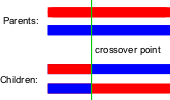
\includegraphics{crossover_single_point}
          \caption{Cruzamento de um ponto}
        \end{figure}
      \item[Cruzamento de múltiplos pontos]
        Diversos pontos são escolhidos e os dados anteriores e posteriores a eles geram novos filhos
        \begin{figure}[!ht]
          \centering
          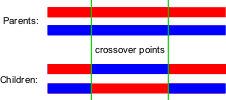
\includegraphics{crossover_multiple_points}
          \caption{Cruzamento de múltiplos pontos}
        \end{figure}
      \item[Cruzamento uniforme]
        Esse tipo de cruzamento utiliza uma taxa de cruzamento que decide qual pai contribuirá com cada gene dos filhos. 
        Isso permite que o cruzamento seja feito a nível de gene enquanto nos operadores de um ou múltiplos pontos é 
        feito por seguimentos.
        \begin{figure}[!ht]
          \centering
          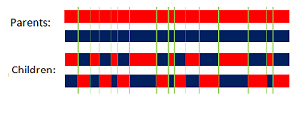
\includegraphics{crossover_uniform}
          \caption{Cruzamento uniforme}
        \end{figure}
    \end{description}

    \subsubsection{Mutação}
    Existem diversos operadores de mutação podendo-se destacar:
    \begin{description}
      \item[Mutação de um ponto] 
        \begin{figure}[!ht]
          \centering
          \includegraphics{mutation_single_point}
          \caption{Mutação de um ponto}
        \end{figure}
      \item[Mutação de múltiplos pontos]

        \begin{figure}[!ht]
          \centering
          \includegraphics{mutation_multiple_points}
          \caption{Mutação de múltiplos pontos}
        \end{figure}
      \item[Mutação uniforme]

        \begin{figure}[!ht]
          \centering
          \includegraphics{mutation_uniform}
          \caption{Mutação uniforme}
        \end{figure}
    \end{description}
    
\subsection{Algorítmos Genéticos Adaptativos (AGA)}
Lorem ipsum...